% fig_hil_roadmap.tex — HIL validation roadmap (Gantt-style)
% Compile: pdflatex fig_hil_roadmap
\documentclass[tikz,border=4pt]{standalone}
\usepackage{tikz}
\usetikzlibrary{positioning,arrows.meta,backgrounds,patterns}
\usepackage{xcolor}

\begin{document}
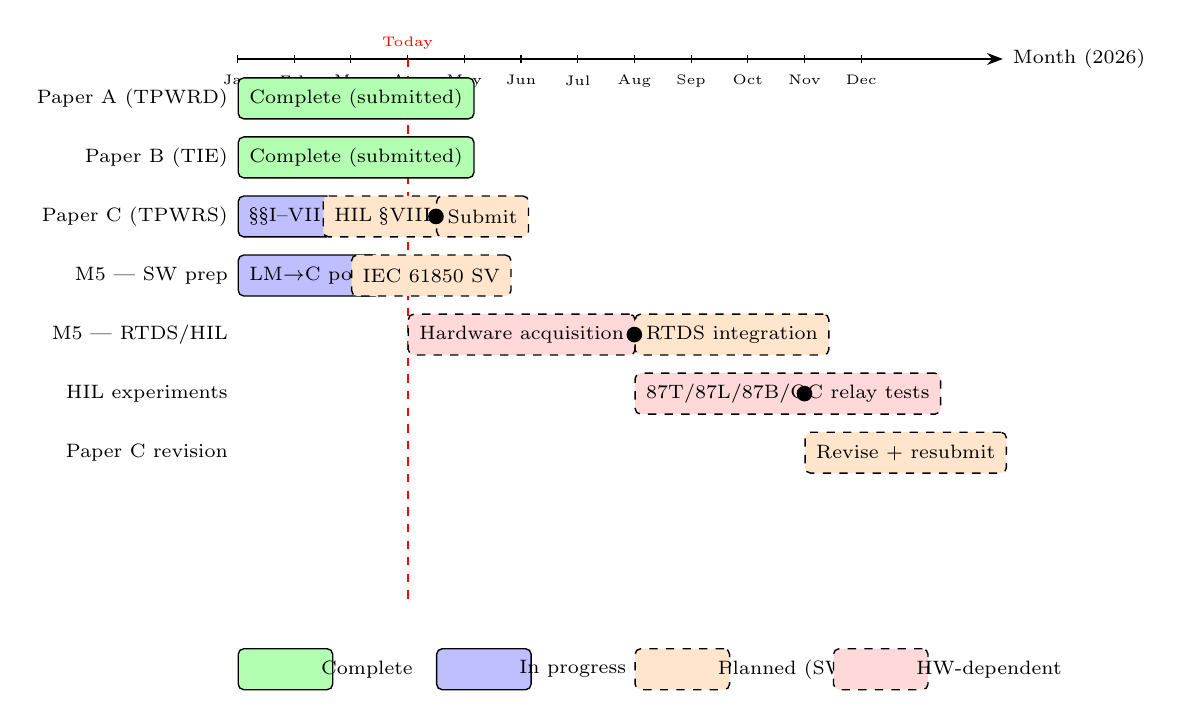
\begin{tikzpicture}[
  font=\small,
  bar/.style={minimum height=0.52cm, draw, rounded corners=2pt,
              line width=0.5pt, align=left, anchor=west,
              inner xsep=4pt, inner ysep=0pt, font=\scriptsize},
  done/.style={bar, fill=green!30},
  active/.style={bar, fill=blue!25},
  planned/.style={bar, fill=orange!20, dashed},
  hw/.style={bar, fill=red!15, dashed},
  milestone/.style={circle, fill=black, inner sep=2pt},
  label/.style={font=\scriptsize, anchor=east},
]

% ---- Time axis (months from Jan 2026) ---------------------------------------
\def\xs{0.72}   % x scale: 1 unit = 1 month
\def\yrow{0.75} % row spacing

% Draw x-axis
\draw[-{Stealth},line width=0.6pt] (0,-0.25) -- (13.5*\xs,-0.25)
  node[right,font=\scriptsize]{Month (2026)};

% Month ticks
\foreach \m/\lbl in {0/Jan,1/Feb,2/Mar,3/Apr,4/May,5/Jun,
                     6/Jul,7/Aug,8/Sep,9/Oct,10/Nov,11/Dec}{
  \draw[line width=0.4pt] (\m*\xs,-0.3) -- (\m*\xs,-0.2);
  \node[font=\tiny,below=1pt] at (\m*\xs,-0.3) {\lbl};
}

% Today marker (April 2026 = month 3)
\draw[red,line width=0.8pt,dashed] (3*\xs,-0.25) -- (3*\xs,-7.2);
\node[font=\tiny,red,above] at (3*\xs,-0.25) {Today};

% ---- Rows (top to bottom) ---------------------------------------------------
% Row 0: Paper A submission
\node[label] at (0, -1*\yrow) {Paper A (TPWRD)};
\node[done, minimum width=3*\xs cm] at (0,-1*\yrow) {Complete (submitted)};

% Row 1: Paper B submission
\node[label] at (0, -2*\yrow) {Paper B (TIE)};
\node[done, minimum width=3*\xs cm] at (0,-2*\yrow) {Complete (submitted)};

% Row 2: Paper C submission
\node[label] at (0, -3*\yrow) {Paper C (TPWRS)};
\node[active, minimum width=1.5*\xs cm] at (0*\xs,-3*\yrow) {§§I–VII};
\node[planned, minimum width=2*\xs cm] at (1.5*\xs,-3*\yrow) {HIL §VIII};
\node[planned, minimum width=1*\xs cm] at (3.5*\xs,-3*\yrow) {Submit};

% Row 3: M5 software prep
\node[label] at (0, -4*\yrow) {M5 — SW prep};
\node[active, minimum width=2*\xs cm] at (0,-4*\yrow) {LM$\to$C port};
\node[planned, minimum width=2*\xs cm] at (2*\xs,-4*\yrow) {IEC 61850 SV};

% Row 4: M5 HIL procurement
\node[label] at (0, -5*\yrow) {M5 — RTDS/HIL};
\node[hw, minimum width=4*\xs cm] at (3*\xs,-5*\yrow) {Hardware acquisition};
\node[planned, minimum width=3*\xs cm] at (7*\xs,-5*\yrow) {RTDS integration};

% Row 5: HIL experiments
\node[label] at (0, -6*\yrow) {HIL experiments};
\node[hw, minimum width=5*\xs cm] at (7*\xs,-6*\yrow) {87T/87L/87B/OC relay tests};

% Row 6: Paper C revision / resubmit
\node[label] at (0, -7*\yrow) {Paper C revision};
\node[planned, minimum width=2*\xs cm] at (10*\xs,-7*\yrow) {Revise + resubmit};

% ---- Milestone diamonds -----------------------------------------------------
\node[milestone] at (3.5*\xs, -3*\yrow) {};   % Paper C §§I–VII complete
\node[milestone] at (7*\xs,   -5*\yrow) {};   % RTDS available
\node[milestone] at (10*\xs,  -6*\yrow) {};   % HIL experiments done

% ---- Legend -----------------------------------------------------------------
\node[done,   minimum width=1.2cm, anchor=west] at (0*\xs, -8.0) {};
\node[anchor=west, font=\scriptsize] at (1.3*\xs, -8.0) {Complete};
\node[active, minimum width=1.2cm, anchor=west] at (3.5*\xs, -8.0) {};
\node[anchor=west, font=\scriptsize] at (4.8*\xs, -8.0) {In progress};
\node[planned,minimum width=1.2cm, anchor=west] at (7.0*\xs, -8.0) {};
\node[anchor=west, font=\scriptsize] at (8.3*\xs, -8.0) {Planned (SW)};
\node[hw,     minimum width=1.2cm, anchor=west] at (10.5*\xs,-8.0) {};
\node[anchor=west, font=\scriptsize] at (11.8*\xs,-8.0) {HW-dependent};

\end{tikzpicture}
\end{document}
